\section{Evaluation}\label{sec:results}

%In this section, we will present our evaluation results of the \systemname. 
We evaluated \systemname~with comprehensive laboratory studies.
We collected from volunteer participants accelerometer sensor readings with Google Glass.
We analyzed these traces offline on a PC.
Our evaluations are primarily aimed at determining the accuracy of detecting 
and differentiating users based on their head-movements, and understand 
the effect of design parameters such as length of the music cue and training 
data-set size, on accuracy. We also report the response time of our Google 
Glass implementation of \systemname.
Our studies were approved by the Institutional Review Board (IRB) of our 
institution.
%based on profiling the execution time of each key 
%functions associated with \systemname, on the Google Glass device.

\iffalse
We conducted extensive evaluation of the Headbanger system. In particular, our 
evaluation focused on showing that a user's body movement pattern can be used 
to establish the user's identify. We first show that even a simple movement 
pattern is hard to imitate by others (i.e., being distinctive), and next show 
that people can easily repeat their own patterns (i.e., being repeatable). To 
conduct the evaluation, we prototyped the Headbanger system using the Google 
Glass, but our system can be easily implemented on other platforms.
\fi

%\begin{figure}[t]
%\centering
%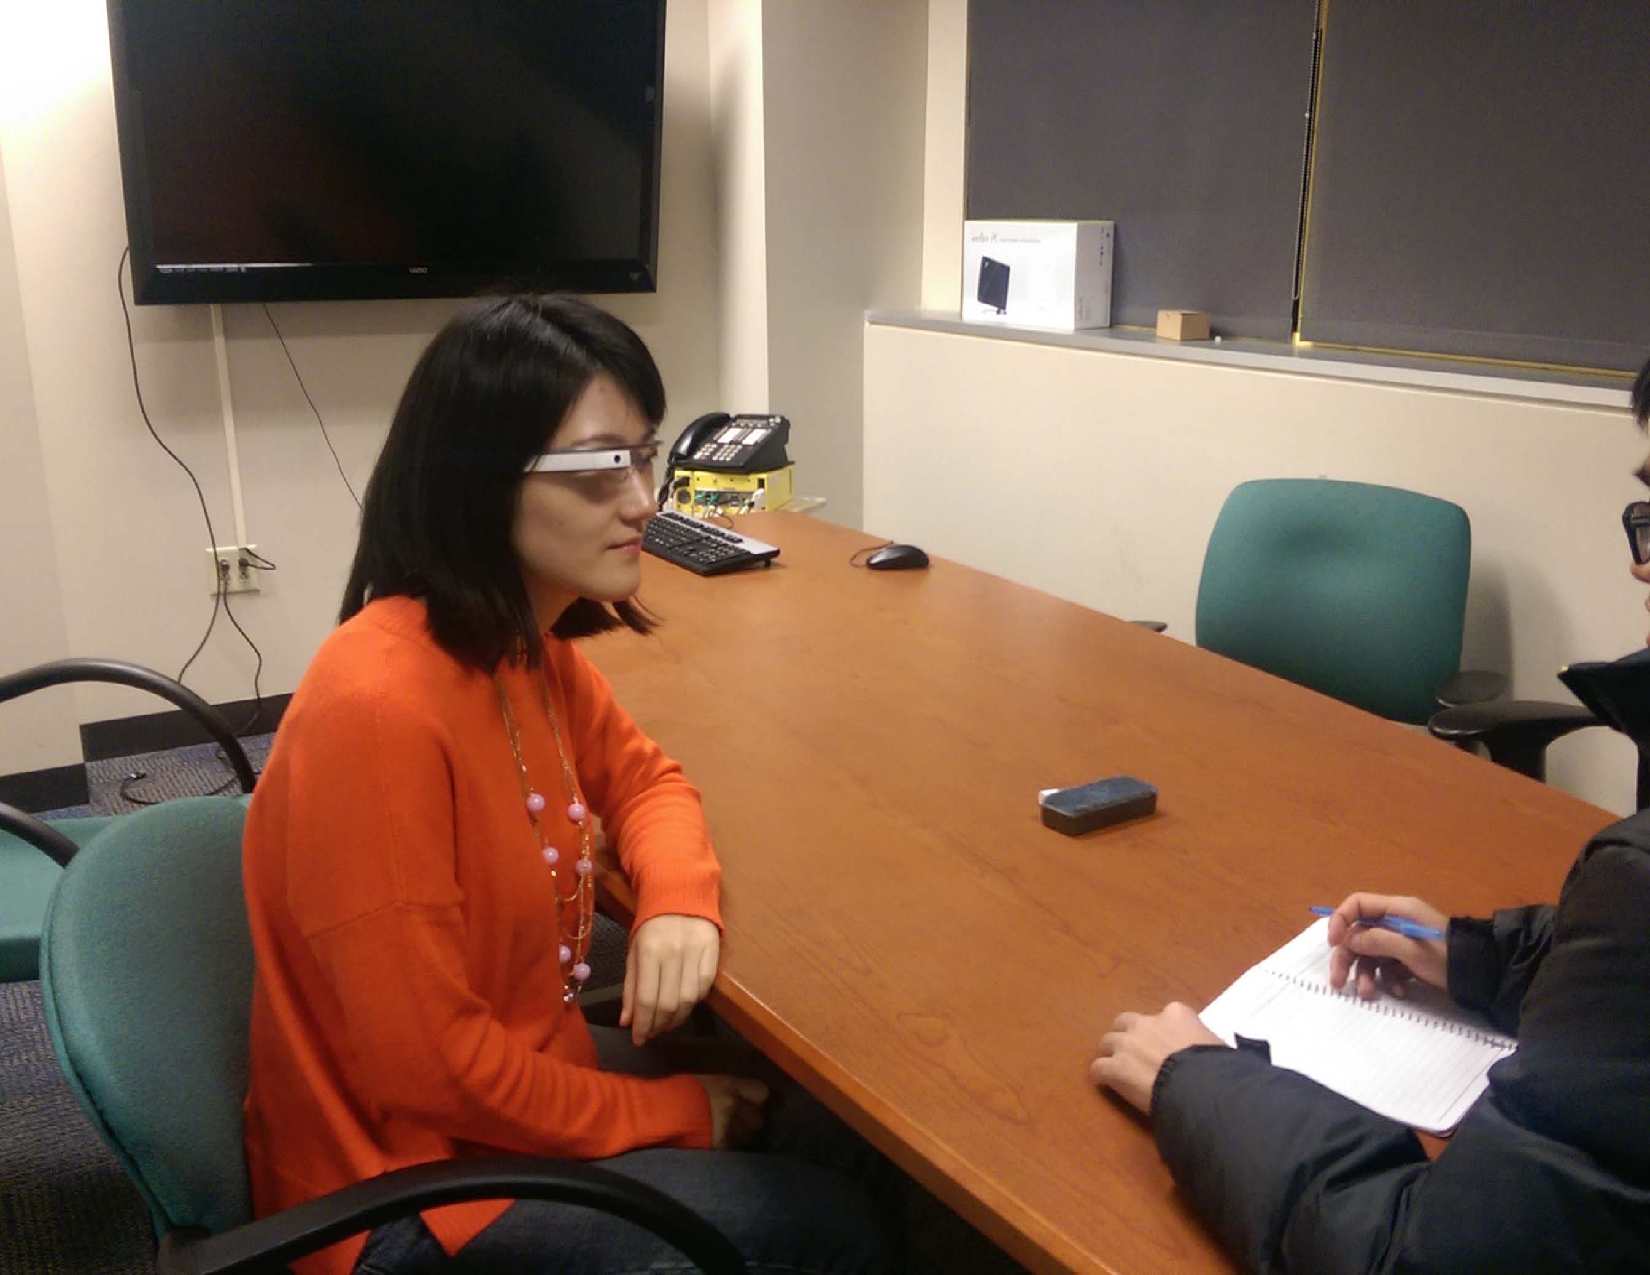
\includegraphics [width=.75\columnwidth]{../fig/exp.pdf}
%\caption{Our team member was collecting data with one of the participants. \label{fig:exp}}
%\end{figure}

\subsection{Method}
%\subsection{Dataset}

\paragraph{Participants}

We had total of 30 volunteer participants. One of them were 
from our list of authors and 29 were other volunteers. 
Table~\ref{tab:human-subjects-distrib} shows the distribution of the age and 
gender of the participants.
The experiments were conducted by one of the non-experimenting authors. 

\paragraph{Procedure}
Our experiment setup primarily aimed at emulating the typical usage scenario 
of the \systemname for authentication, where a user conducts head-movements in 
response to a music cue played on the Google Glass device during the login 
attempt.
In our experiment, all participants were asked to wear a Google Glass 
device. The device ran our data-collection app that played a piece of music 
(music cue), and recorded the accelerometer sensor readings. 
The duration

further, the 
The sensor 
readings were recorded into a text 
file that was stored 
in the Glass's memory and later transported to a PC and analyzed offline 
through a Python script. The experiment was conducted in an well-lit indoor 
academic laboratory environment. 

%During the course of the experiment the 
%experimenter was sitting on a chair and was mostly stationary, where the most 
%significant movements were through head-movements.

%\subsection{Data collection from Human subjects}
 
The participants were allowed to take a break or withdraw from the 
experimentation if they felt uncomfortable at any point; for example, feeling 
dizzy after head-movement for a period of time, not being able to see clearly 
if near-sighted, etcetera. The proctor also allowed the user to take a break 
of about one minute after each experiment trial.

Each trial lasted for the duration of the music piece played on the Glass, and 
we conducted 40 trials for each of the 30 subjects. 
We collected three sets of data traces that correspond to 3, 5 and 10sec of 
the music piece played on the Glass and analyzed offline to evaluate the 
performance of our system.
%After every 5 recording sessions, we asked the subject 
%to take a break to relax their muscle and regain energy. 
%The subjects, 12 females and 9 males, had an average age of 26 
%years.
We will now discuss the evaluation results in detail.

%We asked the subjects to wear the Google Glass and make head-movements while 
%listening to the music track. Meanwhile, we recorded the raw accelerometer 
%data.  Each recording session was 10 seconds long, and we sat through each 
%session with the subject to help him/her use the system properly, as shown in 
%Figure~\ref{fig:exp}. 
\subsection{Accuracy}

\begin{table}[h]
\begin{tabular}{llll}
\hline
\multicolumn{1}{|l|}{Method/System} & \multicolumn{1}{l|}{Headbanger} & 
\multicolumn{1}{l|}{Gafurov et al~\cite{gafurov2006biometric}} & 
\multicolumn{1}{l|}{Derawi et al.~\cite{derawi2010improved}} \\ 
\hline
Sen}sor Location               \multicolumn{1}{l|}{l      & 
H\multicolumn{1}{|l|}{Sensor Location} & \multicolumn{1}{l|} 
{head                            & Lower 
leg}                          &                               
\multicolumn{1}{l|}{left hip}     \\ \hline
\multicolumn{1}{|l|}{EER}           & \multicolumn{1}{l|}{3.47}       & 
\multicolumn{1}{l|}{5}             & \multicolumn{1}{l|}{5.7}           \\ 
\hline
\end{tabular}
\caption{PLACE HOLDER : EERs for different behavioral biometric authentication 
systems}
\end{table}

\subsubsection{Usability for Authentication}

\subsection{Micro-benchmarking}
\subsubsection{Impact of Training set size}
\subsubsection{Number of subjects}

\subsection{Google Glass Implementation}

\subsection{Even Simple Body Movement is Hard to Imitate}\label{sec:experimenr2}
In the first set of experiments, we show that even simple body movement is very hard to imitate by others, and thus body movement is rather distinctive among different people.

\subsubsection{Experimental Setup}
One of the simplest body movement patterns that can be easily captured by built-in sensors is nodding, which we employed in this set of experiments.

Each $ACC$ sample was collected for the duration of 10 seconds. When calculating the classification results, we generated shorter samples of varying lengths (2 seconds, 3 seconds, 6 seconds, and 10 seconds) from the original 10-second samples. The sum of the sample duration and the subsequent processing latency thus determines the authentication response time of our system. Longer sample durations likely lead to more accurate classification results, but shorter sample durations may be preferred by users due to faster authentication responses.

In this set of experiments, we have one glass owner, who designed the nodding pattern,  and 15 imitators who imitated the movement. We collected 100 10-second $ACC$ samples from the owner, during the course of 60 days (from 10/1/2014 to 11/30/2014), ensuring the owner's sensor data includes sufficient variation that naturally occurs with time. We also made a great deal of effort to make sure the imitators accurately imitate the owner's movement -- the owner carefully explained his movement pattern to each imitator, and sat through each data collection session for all the 15 imitators to make sure their movement pattern looks the same to the owner's eye. For reach imitator, we collected 40 10-second $ACC$ samples.

\iffalse
\begin{table}[b]
\small
{\bf Summary}\begin{tabular}{|l||l|l|l||l|l|l|}\hline
& \multicolumn{3}{|c||}{2}& \multicolumn{3}{|c|}{3}\\\cline{2-7}
Sample duration (s)& FRR & FAR & BAC & FRR & FAR & BAC\\
&(\%) &(\%) &(\%) &(\%) &(\%) &(\%)\\\hline

SVM Top 1                 & 25.0 & 16.74 &79.12 & 15.0 & 14.05 & 85.47  \\\hline
SVM Top 3 Voting          & 14.84& 9.24 & 87.95 & 18.48 & 6.85 & 87.33  \\\hline\hline

& \multicolumn{3}{|c||}{6}& \multicolumn{3}{|c|}{10}\\\cline{2-7}
Sample duration (s)& FRR & FAR & BAC & FRR & FAR & BAC\\
&(\%) &(\%) &(\%) &(\%) &(\%) &(\%)\\\hline

SVM Top 1                   & 3.33& 6.66& 95.0  & 0.0& 9.62& 95.18 \\\hline
SVM Top 3 Voting            & 7.27& 6.17& 93.27 & 4.84& 6.17& 94.48 \\\hline

\end{tabular}
\caption{Average FAR, FRR, and BAC for SVM-based classification when we choose different 4 imitators in the training set (from the total 15 imitators). We have the results for different sample durations. In these results, we use the earliest 40 owner samples in the training set.\label{tab:kfoldfalse-svm}}
\end{table}
\fi

\iffalse
\begin{table}[b]
\small
\begin{tabular}{|l||l|l|l||l|l|l|}\hline
& \multicolumn{3}{|c||}{2}& \multicolumn{3}{|c|}{3}\\\cline{2-7}
Sample duration (s)& FRR & FAR & BAC & FRR & FAR & BAC\\
&(\%) &(\%) &(\%) &(\%) &(\%) &(\%)\\\hline

SVM Top 1                   & & &83.64 & & & 87.11  \\\hline
SVM Top 3 Voting            & & & 84.90 & & & 88.96 \\\hline\hline

& \multicolumn{3}{|c||}{6}& \multicolumn{3}{|c|}{10}\\\cline{2-7}
Sample duration (s)& FRR & FAR & BAC & FRR & FAR & BAC\\
&(\%) &(\%) &(\%) &(\%) &(\%) &(\%)\\\hline

SVM Top 1                   & & & 90.68 & & & 92.63 \\\hline
SVM Top 3 Voting            & & & 91.38 & & & 93.02 \\\hline

\end{tabular}
\caption{Average FAR, FRR, and BAC for SVM-based classification when we choose different 40 owner samples in the training set (from the total of 100 samples).  We have the results for different sample durations. In these results, we use the first four imitators in the training set.\label{tab:kfoldtrue-svm}}
\end{table}
\fi

\subsubsection{Classification Metrics}
In this study, we consider both SVM based classification and thresholding based classification. The classification process is different for these two approaches:

\begin{itemize}
\item \emph{SVM based classification.} For SVM based classification, we need to construct a training set that consists of both true training data (from the owner) and false training data (from the imitators). In total, we have 100 data samples from the owner and $15 \times 40$ samples from imitators, from which we include $S$ samples from the owner, and all the samples from $I$ imitators ( $I \times 40$ samples) in the training set. Therefore, we have $100-S$ owner samples, and $(15-I)\times 40$ imitator samples in the testing set.


\item \emph{Thresholding based classification.} For thresholding based classification, the training set only consists of data samples from the owner. Similar to the SVM case, we use $S$ samples from the owner as the training set, and all the other samples as the test data.
\end{itemize}

In our evaluation, the default value for $S$ is 40, and the default value for 
$I$ is 4. In the evaluation, we varied the value of $S$ and $I$ as well as the 
chosen training samples to ensure the robustness of our system.
%~\footnote{In the interest of space, we didn't include the results with 
%different I values in this paper.}.

For both SVM-based and thresholding-based classification approaches, we consider two testing methods. The first method involves comparing the test sample against the top 1 training sample from a user, which we refer to as \emph{Top 1} testing. The second method involves comparing the test sample against the top 3 training samples from a user and then determining the classification result by voting among these three results, which we refer to as \emph{Top 3 Voting} testing.

In this study, we consider classification metrics that are popular in biometric authentication, namely false acceptance rate $FAR$ (the percentage of false test samples that are mistakenly accepted) and false rejection rate $FRR$ (the percentage of true test samples that are mistakenly rejected). Usually, an overly strict classification system leads to high $FRR$, while an overly relaxed system leads to high $FAR$. We also consider balanced accuracy $$BAC = 1 - (FAR+FRR)/2,$$ which is a combined metric that measures both $FAR$ and $FRR$.


\iffalse
\subsubsection{SVM Classification Results}

As mentioned earlier, SVM classification requires training data from both the owner and imitators. In the results shown in Table~\ref{tab:kfoldfalse-svm}, we used the earliest 40 samples from the owner (out of 100 total owner samples), but varied the imitators that are included in the training set. Specifically, if we label the 15 imitators as $I_1, ..., I_{15}$, then we had the following 15 different combinations of imitators in the training set: $\{I_1, I_2, I_3, I_4\}$, $\{I_2, I_3, I_4, I_5\}$, $\dots$, $\{I_{15}, I_1, I_2, I_3\}$.  Table~\ref{tab:kfoldfalse-svm} shows the average FAR, FRR, and BAC values over these 15 combinations. By considering these different cases, we can eliminate the impact of having a specific imitator in the training data and the results are more representative. Here, we also vary the sample duration: 2, 3, 6, and 10 seconds.

From Table~\ref{tab:kfoldfalse-svm}, we have the following main observations:
\fi

\begin{enumerate}
\item \emph{Even simple nodding is not easy to imitate: nodding for 6 seconds can classify 95\% of the users.} As the sample duration increases from 2 seconds to 6 seconds, the classification accuracy improves significantly -- the BAC value changes from 79.12\% to 95\% for top 1 testing, and from 87.95\% to 93.27\% for top 3 voting. After the sample duration reaches 6 seconds, the improvement becomes less pronounced. This suggests that a sample duration of 6 seconds is sufficient to successfully classify 95\% of the users. We feel that moving our head gently along with music for 6 seconds is in general not a cumbersome process for most users. It further suggests that even simple nodding is hard to imitate by others, and thus head-movement has the potential to serve as a reliable biometric characteristic for smart wearable authentication.


\item \emph{For sample duration of 6 seconds, testing against 1 training sample is sufficient.} The results also show that, when the sample duration is short (e.g., 2 or 3 seconds), comparing the test sample against top 3 training samples leads to much better classification result. When the sample duration is reasonably long, say 6 seconds, comparing the test sample against the top 1 training sample leads to better results. This is advantageous because top 1 testing incurs much less processing and energy overhead, lending itself for execution on wearable devices.
\end{enumerate}

\iffalse
\begin{figure*}[t]
\centering
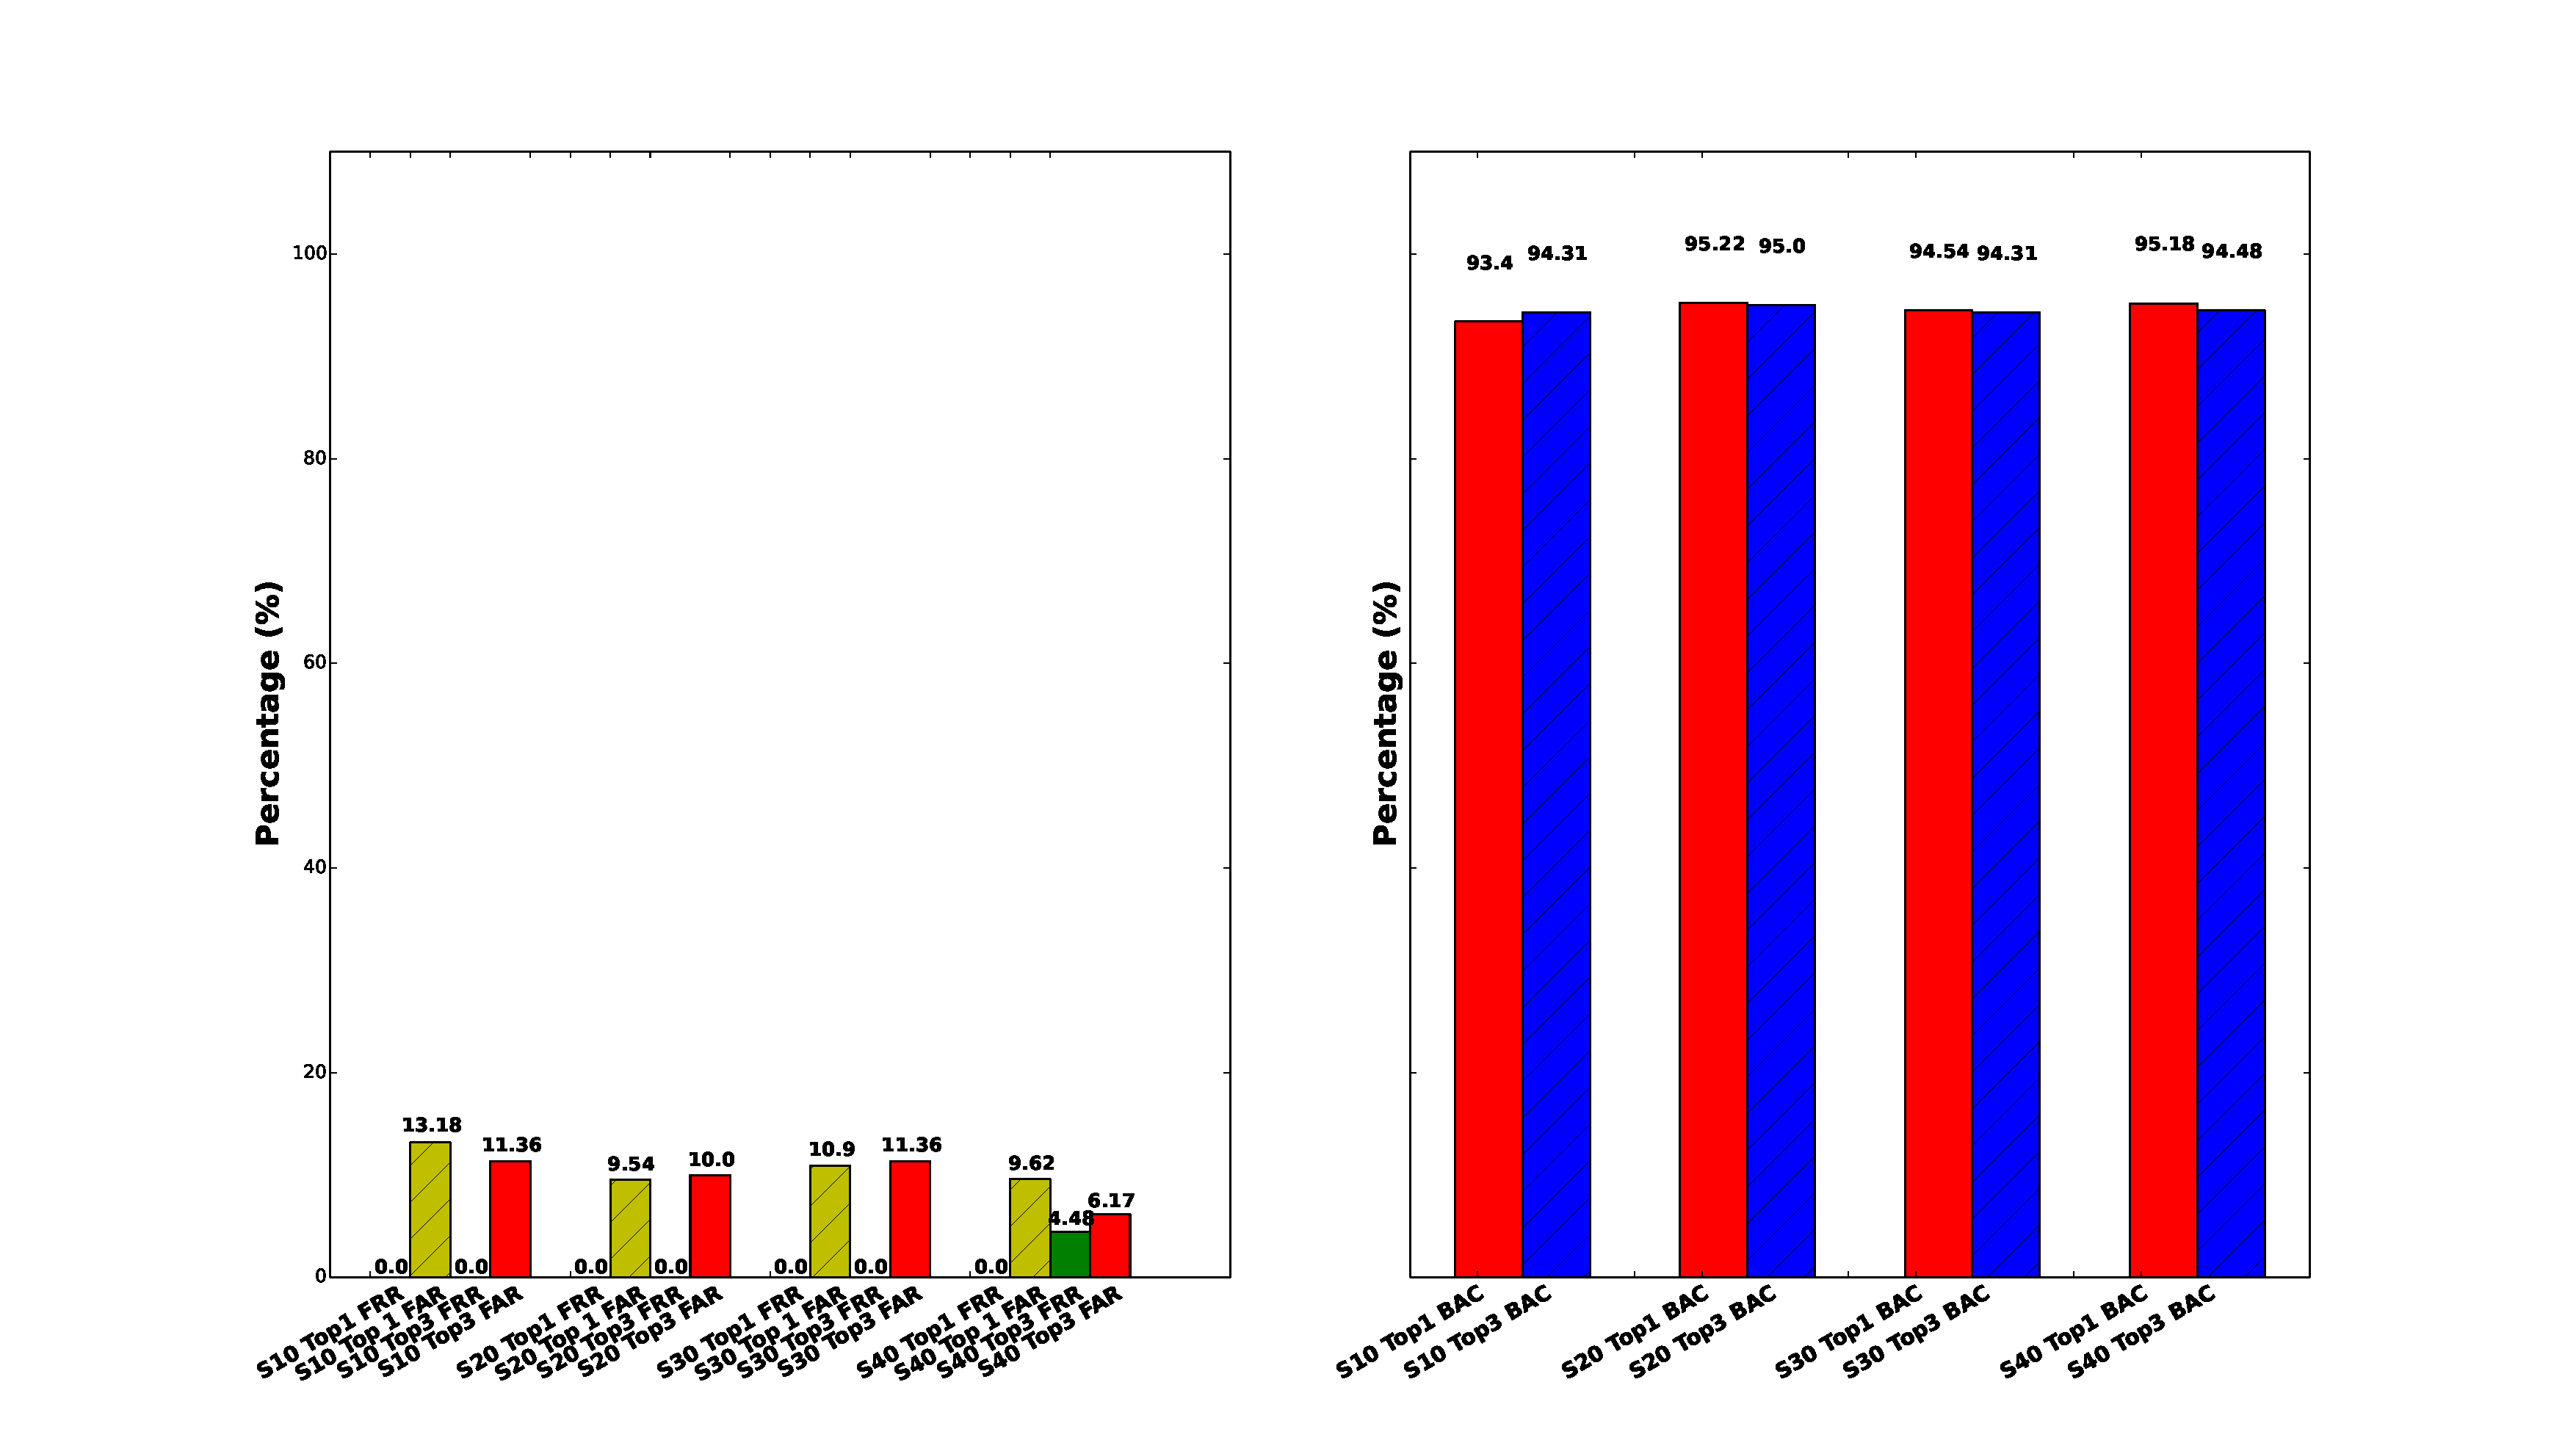
\includegraphics [width=.95\linewidth]{../fig/exp1_vary_size_svm}
\caption{In this set of experiments, we studied whether the number of owner 
samples in the training set has a bearing on the SVM classification results. 
(a) shows the FRR and FAR results for each scenario, and (b) shows the BAC 
results.\label{fig:exp1_vary_size_svm}}
\end{figure*}
\fi

\vspace{4pt}\textbf{The Impact of Training Dataset Size:} Next we studied whether the number of owner samples in the training set has a bearing on the SVM classification results. We varied the number of owner training samples as 10, 20, and 30, and show the resulting FRR and FAR values in Figure~\ref{fig:exp1_vary_size_svm}(a) and BAC results in Figure~\ref{fig:exp1_vary_size_svm}(b). Note that we have in total 100 samples from the owner.

From the results, we observe that there is no clear trend when we vary the number of owner samples in the training set. When we increase the owner training samples from 10 to 20, the average BAC value increased, but only very marginally. This result suggests that to make the classification light-weight, thus suitable for wearable devices, we can use a small number of training set without hurting the performance.


\subsubsection{Thresholding-Based Classification}
\iffalse
\begin{table}[b]
\small
\begin{tabular}{|l||l|l|l||l|l|l|}\hline
& \multicolumn{3}{|c||}{2}& \multicolumn{3}{|c|}{3}\\\cline{2-7}
Sample duration (s)& FRR & FAR & BAC & FRR & FAR & BAC\\
&(\%) &(\%) &(\%) &(\%) &(\%) &(\%)\\\hline

Th Top 1                   & & &92.55 & & & 92.32  \\\hline
Th Top 3 Voting            & & &92.7 & & & 93.31 \\\hline\hline

& \multicolumn{3}{|c||}{6}& \multicolumn{3}{|c|}{10}\\\cline{2-7}
Sample duration (s)& FRR & FAR & BAC & FRR & FAR & BAC\\
&(\%) &(\%) &(\%) &(\%) &(\%) &(\%)\\\hline

Threshold Top 1                   & & & 93.71  & & & 94.69 \\\hline
Threshold Top 3 Voting            & & & 95.53 & & & 95.53 \\\hline

\end{tabular}
\caption{Average FAR, FRR, and BAC for Thresholding-based classification when we choose different 4 imitators in the training set (from the total 15 imitators). We have the results for different sample durations. In these results, we use the earliest 40 owner samples in the training set.\label{tab:kfoldfalse-th}}
\end{table}
\fi


\begin{table}[b]
\small
\begin{tabular}{|l||l|l|l||l|l|l|}\hline
& \multicolumn{3}{|c||}{2}& \multicolumn{3}{|c|}{3}\\\cline{2-7}
Sample duration (s)& FRR & FAR & BAC & FRR & FAR & BAC\\
&(\%) &(\%) &(\%) &(\%) &(\%) &(\%)\\\hline

Th Top 1                   &3.33 & 18.57&89.04 & 5.76& 16.63& 88.8  \\\hline
Th Top 3 Voting            &1.80 & 13.94&92.12 & 1.04& 12.67& 93.14 \\\hline\hline

& \multicolumn{3}{|c||}{6}& \multicolumn{3}{|c|}{10}\\\cline{2-7}
Sample duration (s)& FRR & FAR & BAC & FRR & FAR & BAC\\
&(\%) &(\%) &(\%) &(\%) &(\%) &(\%)\\\hline

Th Top 1                   & 3.17& 8.74& 94.05 & 1.34& 1.99& 98.33 \\\hline
Th Top 3 Voting            & 5.63& 9.15& 92.60 & 1.42& 4.78& 96.89 \\\hline

\end{tabular}
\caption{Average FAR, FRR, and BAC for thresholding-based classification when we choose different 40 owner samples in the training set (from the total of 100 samples).  We have the results for different sample durations. In these results, we use the first four imitators in the training set.\label{tab:kfoldtrue-th}}
\end{table}

\begin{figure*}[t]
\centering
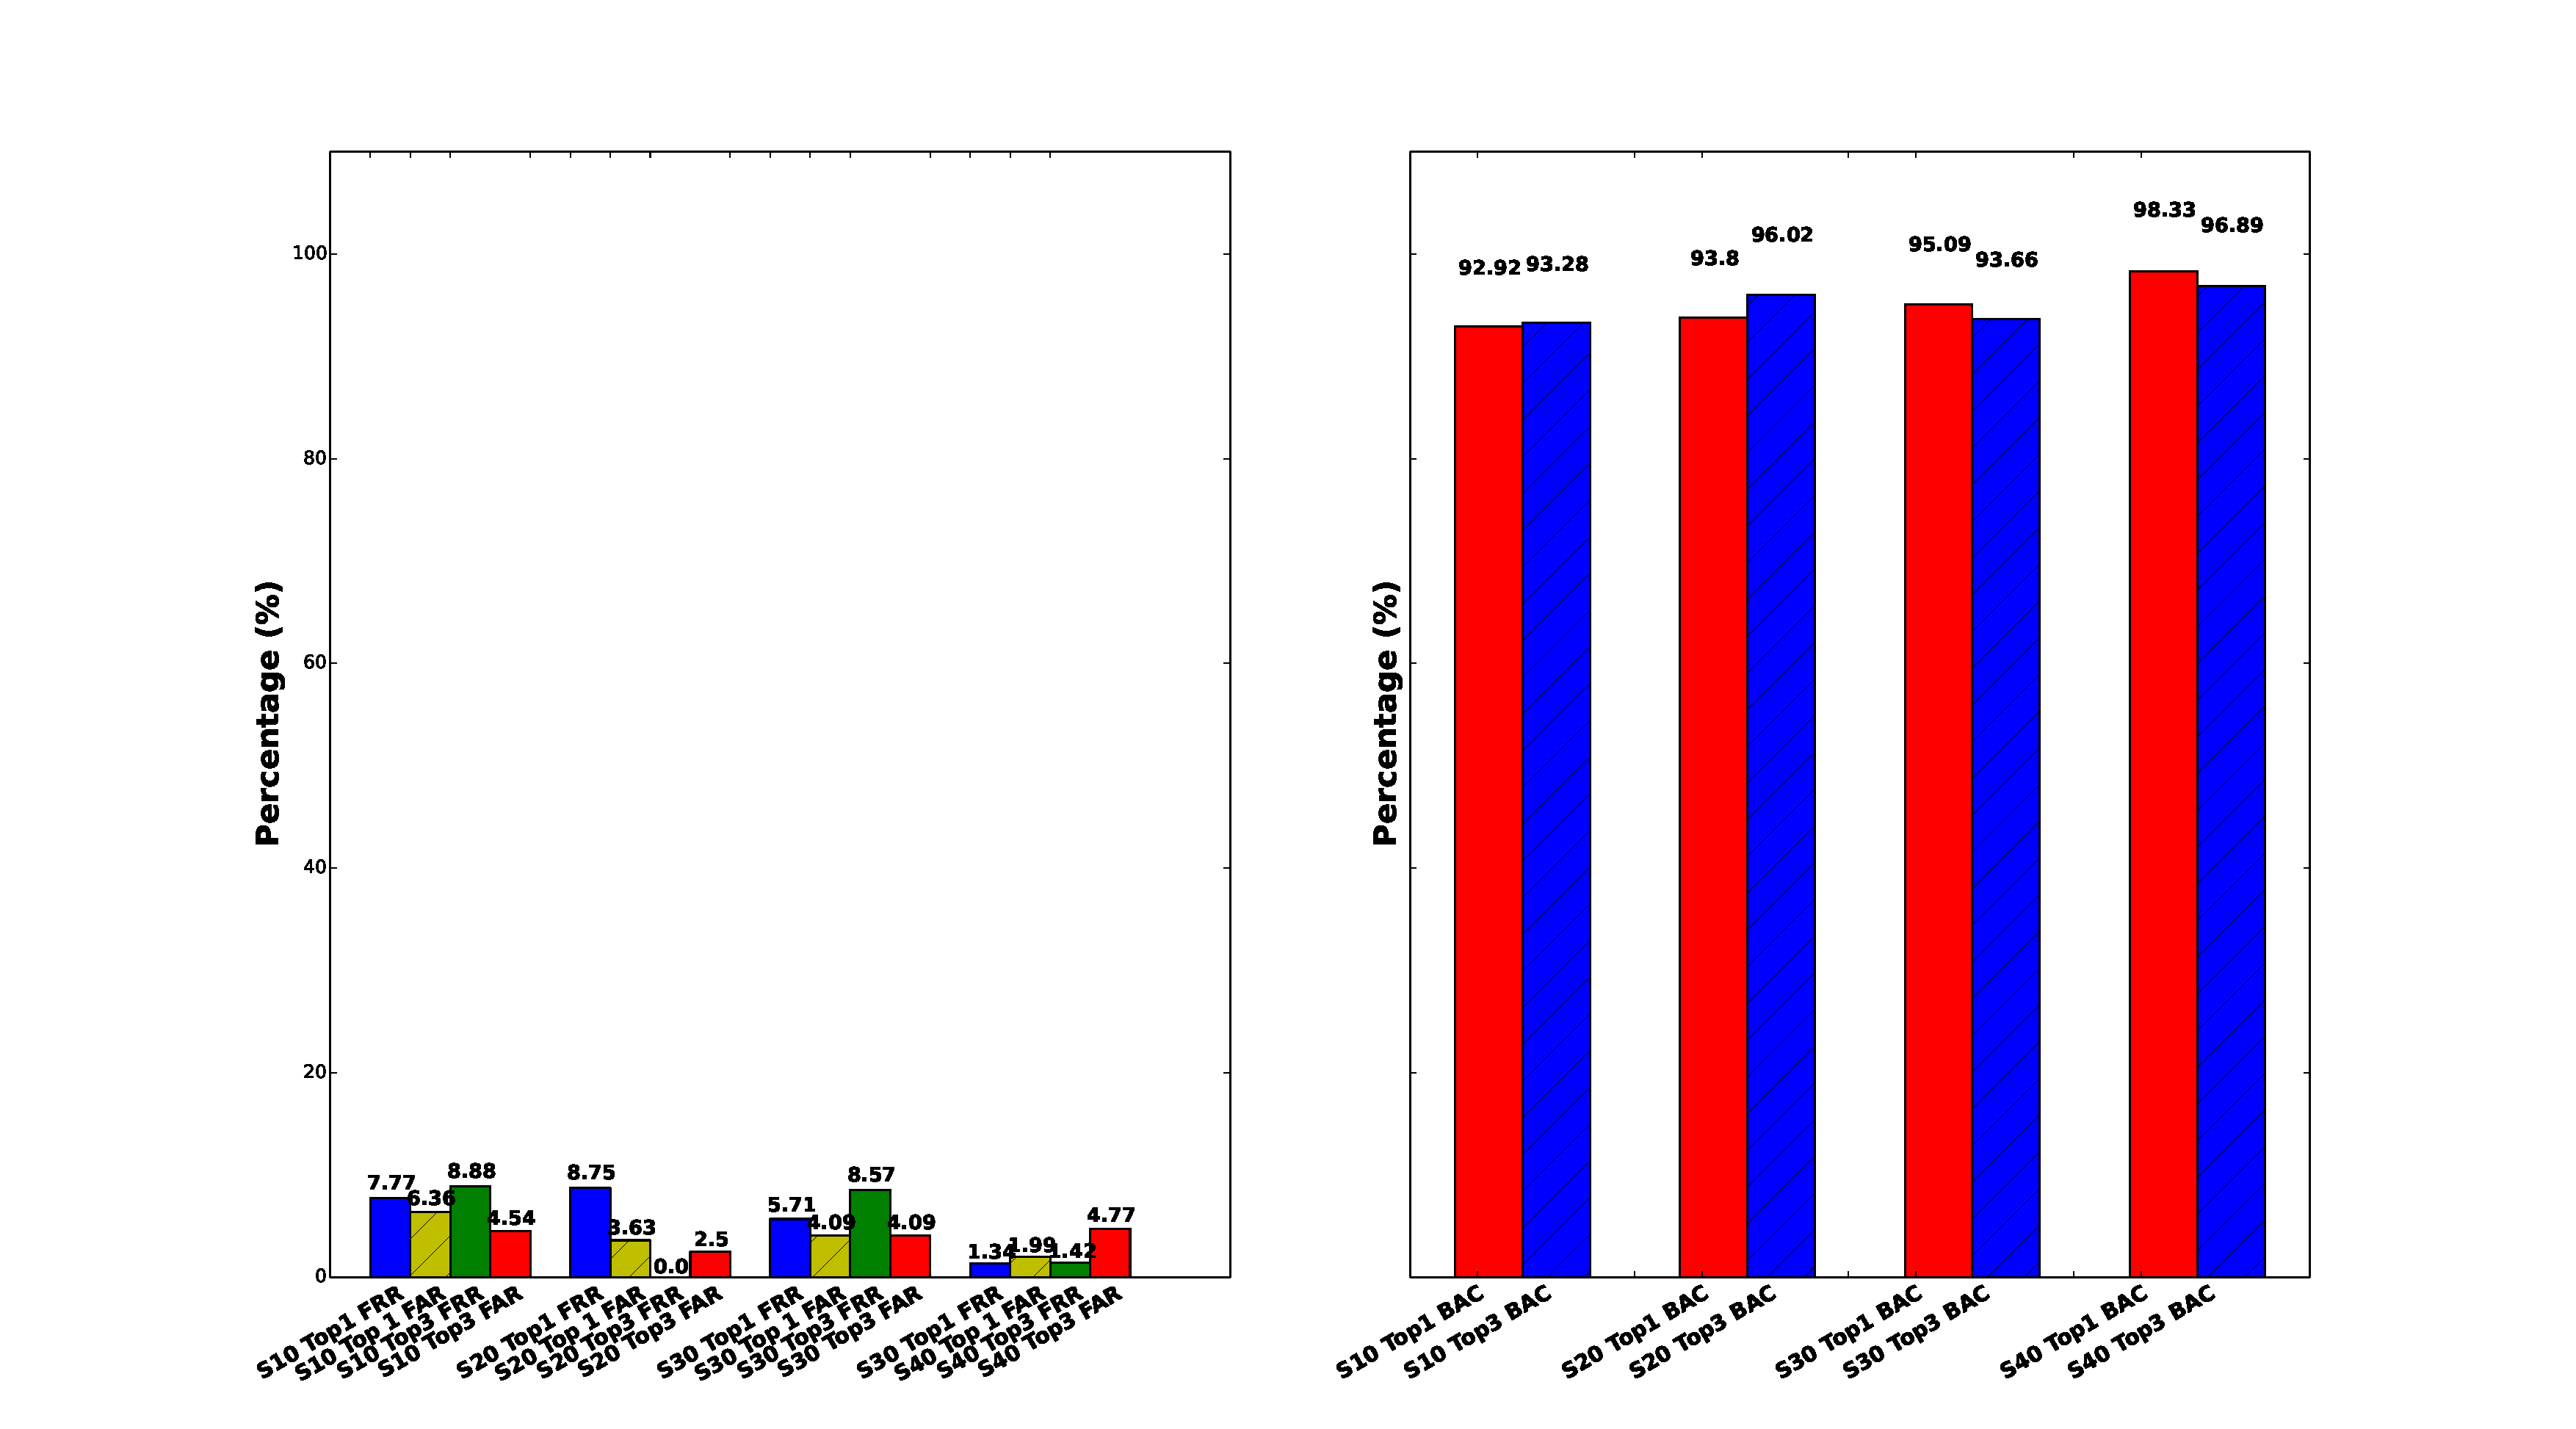
\includegraphics [width=.95\linewidth]{../fig/exp1_vary_size_thre.eps}
\caption{In this set of experiments, we studied whether the number of owner samples in the training set has a bearing on the thresholding classification results. (a) shows the FRR and FAR results for each scenario, and (b) shows the BAC results.\label{fig:exp1_vary_size_th}}
\end{figure*}

\begin{figure*}[t]
\centering
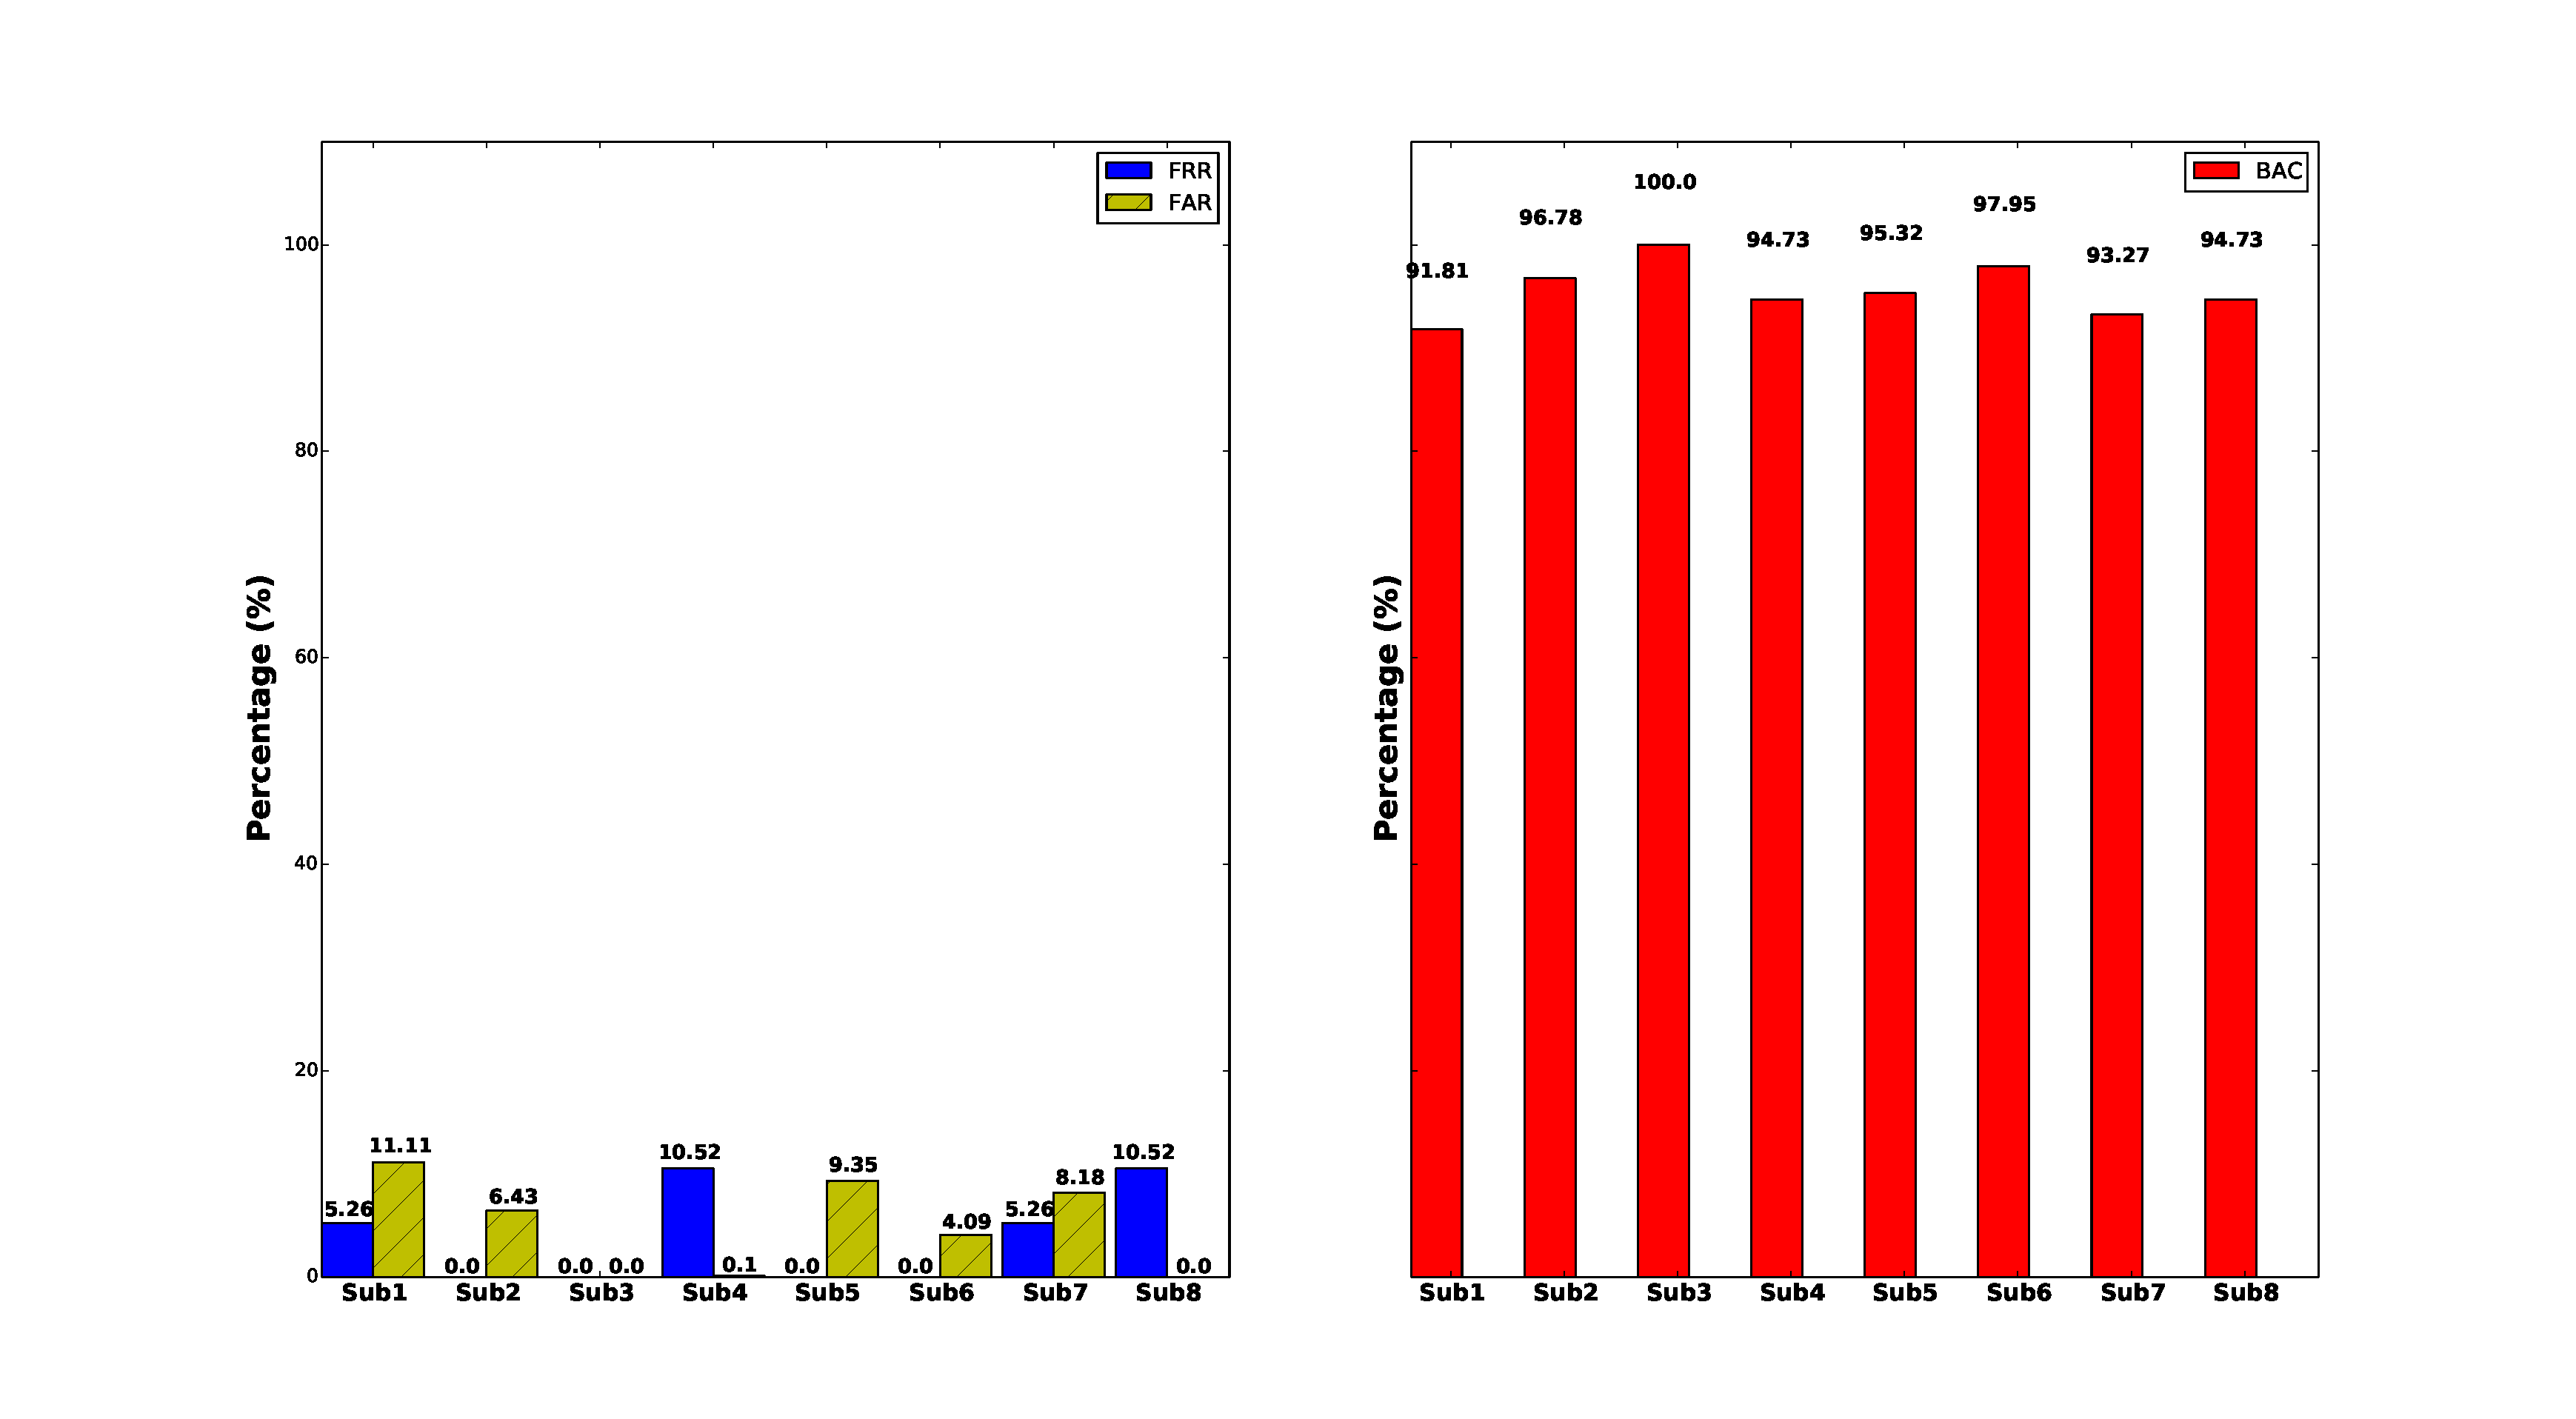
\includegraphics [width=.85\linewidth]{../fig/exp2_frr_far_bac.pdf}
\caption{In this set of experiments, we studied whether a user can successfully repeat her own head-movement pattern. We had 8 subjects, each performing her own choice of head-movement patterns. We collected 38 samples for each subject. (a) shows the FRR and FAR results for each subject, and (b) shows the BAC results. Thresholding-based classification with top 3 voting was used to generate these results. \label{fig:exp2_frr_far_bac}}
\end{figure*}

Thresholding based classification only requires owner samples in the training set. In order to eliminate the impact of choosing certain training samples, we rotate the 40 training samples and summarize the average FAR, FRR, and BAC values in Table~\ref{tab:kfoldtrue-th}. Specifically, if we label the 100 owner samples as $S_1, S_2, ..., S_{100}$, then we ran 100 different experiments in this case, with training set being $\{S_1, S_2, ..., S_{40}\}$, $\{S_2, S_3, ..., S_{41}\}$, $\dots$, $\{S_{100}, S_1, ... S_{39}\}$, respectively.  Here, we also varied the sample duration: 2, 3, 6, and 10 seconds.

From Table~\ref{tab:kfoldtrue-th}, we have the following main observations:

\begin{enumerate}
\item \emph{Thresholding-based classification, though more light-weight, fares better than SVM.} Results in Table~\ref{tab:kfoldtrue-th} show that thresholding-based classification in general fares better than SVM (except the 6-second case). With 10-second sample duration, thresholding-based classification has a BAC value of 98.33\%. This is mainly because the thresholding-based classifier only relies on true training samples, hence more robust against imitators whose movement pattern is similar to that of the owner. This result is desirable because thresholding-based classification is much more light-weight than SVM classification, and thus more suitable for wearable devices.

\item \emph{For sample duration of 6 seconds or longer, comparing against the top 1 sample is sufficient.} We also observe that when the sample duration is 6 seconds or longer, it is preferred to compare the test sample against the top 1 training sample. This can significantly reduce the computation overhead of our system.

\item \emph{Thresholding-based classification has better FRR than FAR values.} Results in Table~\ref{tab:kfoldtrue-th} show that thresholding-based classification always has very low FRR values, even with short sample durations. With sample duration of 2 seconds, the FRR values are 3.33\% for top 1 testing and 1.80\% for top 3 voting, while the FAR values are 18.57\% for top 1 testing and 13.94 for top 3 voting. This suggests that even with short sample durations, thresholding-based classification is good at identifying the pattern of the same user. When the sample duration increases, we observe that the FAR values drop significantly, to as low as 1.99\% for top 1 testing and 4.78\% for top 3 voting for 10-second sample durations.
\end{enumerate}

\vspace{4pt}\textbf{The Impact of Training Dataset Size:} Next we studied whether the number of owner samples in the training set has a bearing on the thresholding classification results. We varied the number of owner training samples as 10, 20, and 30, and show the resulting FRR and FAR values in Figure~\ref{fig:exp1_vary_size_th}(a) and BAC results in Figure~\ref{fig:exp1_vary_size_th}(b). %***YZ: 40??***

Like the case in SVM classification, we didn't see any noticeable change in classification results with respect to the training data set size. This observation is advantageous in that we can reduce the training dataset size to further reduce the processing requirement and power consumption of our system.

\subsection{Head-movement Patterns are Repeatable}
In the second set of experiments, we would like to find out whether a user can successfully repeat her own head movement if each user is asked to come up with their own movement pattern.

\vspace{4pt}\textbf{Classification Results:} In this set of experiments, we had 8 subjects, and for each subject, we collected 38 $ACC$ samples with sample duration of 10 seconds. Each subject performed different head-movement patterns of their choice.

In generating the classification results, we employ a process that involves 8 iterations. In each iteration, we assume the legitimate glass owner is one of the users. We use 19 $ACC$ samples of this user as the training data set, and testing with his/her other 19 $ACC$ samples together with the other 7 user's $ACC$ samples. For each iteration, we calculate the resulting FRR, FAR, and BAC values (using the top 3 voting for thresholding-based classification), and show the results in Figure~\ref{fig:exp2_frr_far_bac}, where Figure~\ref{fig:exp2_frr_far_bac}(a) shows the FRR and FAR values, while Figure~\ref{fig:exp2_frr_far_bac}(b) shows the BAC values.

After carefully examining the results in Figure~\ref{fig:exp2_frr_far_bac}, we have the following main observations:
\begin{enumerate}
\item \emph{Head-movements are highly repeatable.} The first observation is that a user's head-movement pattern is usually highly repeatable. Among the 8 subjects that we studied, the highest BAC value is 100\%, and the lowest is 91.81\%, with the average BAC value of 95.57\%. Overall, this result suggests that the head-movement pattern is a promising biometric candidate for user authentication.

\item \emph{User head-movements have different level of stability.} Even from the small-scale 8 subject study, we found that users have different level of stability in their head-movements; some are much more stable than others. In our example, subject 3 has 0 FRR and 0 FAR, while subject 1 has 5.26\% FRR and 11.11\% FAR. We suspect that through proper training, subjects could improve their stability. However, we didn't test this hypothesis in this study. We also didn't notice any correlation between a user's stability with his/her age or gender.
\end{enumerate}

\begin{figure*}[t]
\centering
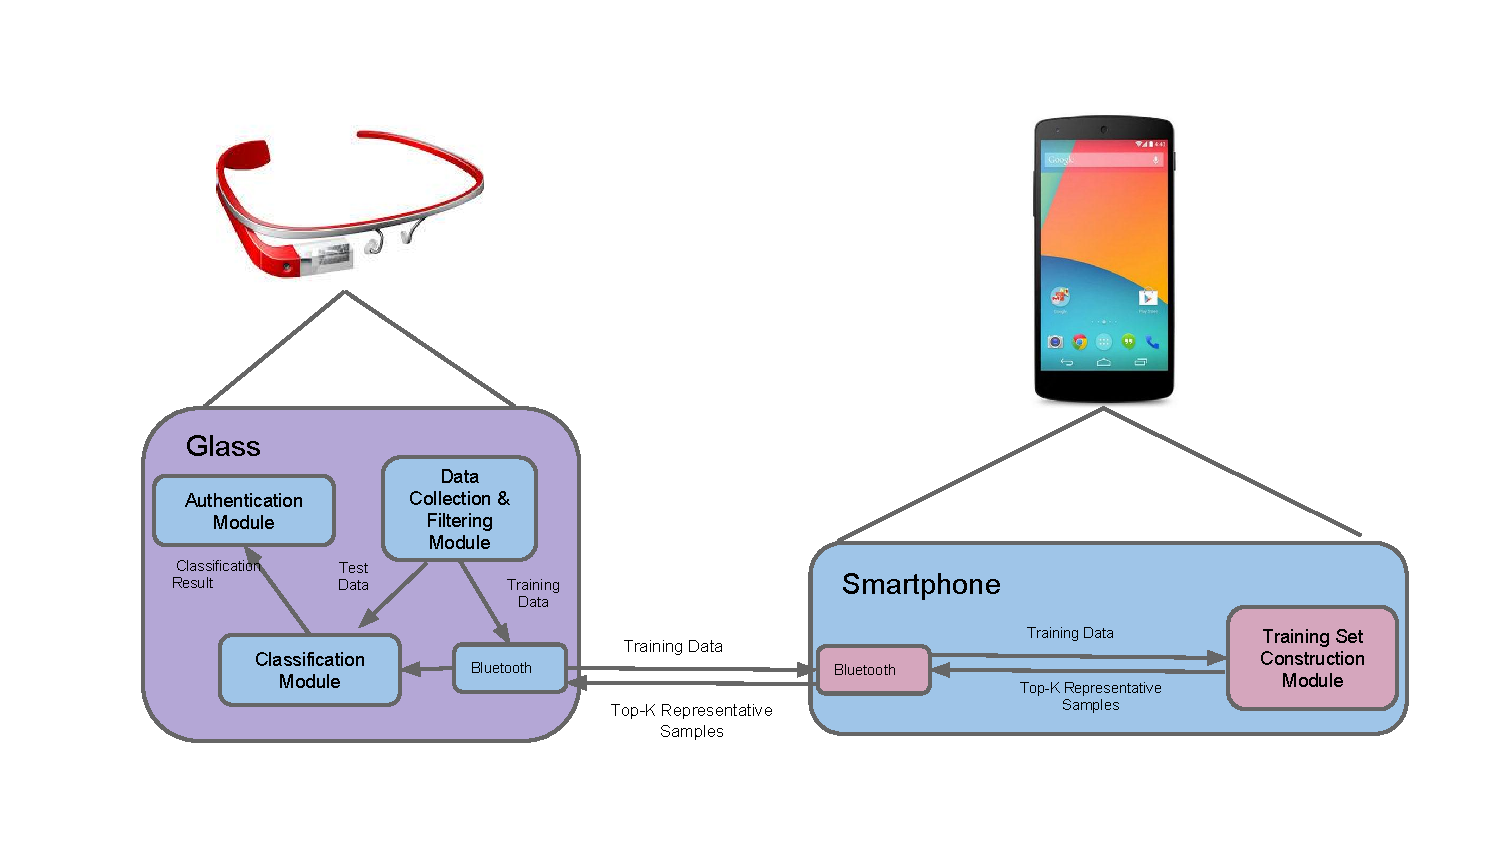
\includegraphics [width=.85\linewidth]{../fig/sofware_architecture}
\caption{The software modules for the Headbanger authentication app. Note that the Training Set Construction Module is executed on the bluetooth-paired smartphone due to its computing intensiveness. \label{fig:software_arch}}
\end{figure*}


\subsection{Headbanger Authentication App Implementation}
We implemented the Headbanger authentication app on Google glass. Figure~\ref{fig:software_arch} shows the software modules the app consists of. Among all the software modules, the ``training set construction model'' is the most computing-intensive, and as a result, we executed the model on the bluetooth-paired smartphone. The rest of the modules are implemented and executed on the glass. In our on-glass app, the classification module runs the thresholding-based classification. Table~\ref{tab:glass} shows the measured processing latency (the time that elapsed between when the test sample is collected and when the authentication result is generated). The results show that even after our aggressive optimizations, the processing latencies are still rather substantial, which suggests that further optimizations are needed.

\begin{table}[b]
\small\centering
\begin{tabular}{|l|l|}\hline
Music sample duration (s) & processing latency (s) \\\hline
2 & 0.84\\\hline
5 & 2.75 \\\hline
10 & 4.47 \\\hline
\end{tabular}
\caption{Measured processing latencies on Google Glass with different sample durations. We generated the results using Top 1 testing for thresholding based classification.\label{tab:glass}}
\end{table}



\iffalse
\subsection{Controlled Experiments: Can You Repeat Your Body Movement?}\label{sec:experiment1}
We first investigate the consistency of the movement performed by each subject. Physical biometric such as fingerprint and iris, which are permanent characteristics that remains regardless environment, emotion, and time. However, behavioral biometric is combined with human controllable movement
\fi

